\documentclass[12pt]{article}
\usepackage{multicol,graphicx}
\usepackage[colorlinks,breaklinks,linkcolor=red,citecolor=blue]
{hyperref} 
\def\sectionautorefname~#1\null{\S#1\null}
\usepackage{charter,amsmath,amssymb,breakurl}
\usepackage{eulervm}
\usepackage[letterpaper,margin=.75in]{geometry}
\def\equationautorefname~#1\null{(#1)\null}
\def\itemautorefname~#1\null{(#1)\null}
\title{Worksheet 2}
\author{}\date{}
\let\ln\relax\DeclareMathOperator{\ln}{\mathsf{ln}}
\let\sin\relax\DeclareMathOperator{\sin}{\mathsf{sin}}
\let\arctan\relax\DeclareMathOperator{\arctan}{\mathsf{arctan}}
\let\cos\relax\DeclareMathOperator{\cos}{\mathsf{cos}}
\let\min\relax\DeclareMathOperator*{\min}{\mathsf{min}}
\let\max\relax\DeclareMathOperator*{\max}{\mathsf{max}}
\let\sup\relax\DeclareMathOperator*{\sup}{\mathsf{sup}}
\let\inf\relax\DeclareMathOperator*{\inf}{\mathsf{inf}}
\let\lim\relax\DeclareMathOperator*{\lim}{\mathsf{lim}}
\everymath{\displaystyle}
\begin{document}
\maketitle
\thispagestyle{empty}

\begin{enumerate}
\item Calculate the partials $f_x$ and $f_y$ where $f$ is each
of the following functions.
\begin{enumerate}
\item $5x^2y^3+8xy^2-3x^2$
\item $\left(x^2+x-y\right)^7$
\item $A^\alpha x^{\alpha+\beta}y^{1-\alpha-\beta}$
\item $xe^{\sqrt{xy}}$
\end{enumerate}

\item Consider the function
\[z=m\left(x-x_0\right)+n\left(y-y_0\right)+z_0\]
\begin{enumerate}
\item Describe the graph of $z$.
\item What is the significance of the point $\left(
x_0,y_0,z_0\right)$?
\item Calculate the partials $\frac{\partial z}{\partial x}$
and $\frac{\partial z}{\partial y}$.
\item How is $z$ analogous to the point-slope form of
a line?
\item Find an equation of the plane tangent to the
graph of $z=2x^2+3y^2$ at the point $\left(1,1\right)$.
\end{enumerate}

\begin{multicols}{2}
\item Consider the function $z=x^{1/3}y^{1/3}$,
shown at the right.
\begin{enumerate}
\item\label{Definition} Calculate the partials
$f_x\left(0,0\right)$ and $f_y\left(0,0\right)$
directly from the definition.
\item What would have happened had you
tried to use the Power Rule
in \autoref{Definition}?
\item Calculate the tangent plane to $z$
at the point $\left(0,0\right)$.
\item\label{NotDiff} A function of two variables is called
{\em differentiable} at $\left(x_0,y_0\right)$ if
it well-approximated by its tangent plane at that point.
Do you think $z$ is differentiable at $\left(0,0\right)$?
\item \autoref{NotDiff} notwithstanding, is $z$
continuous at $\left(0,0\right)$?
\end{enumerate}
\begin{center}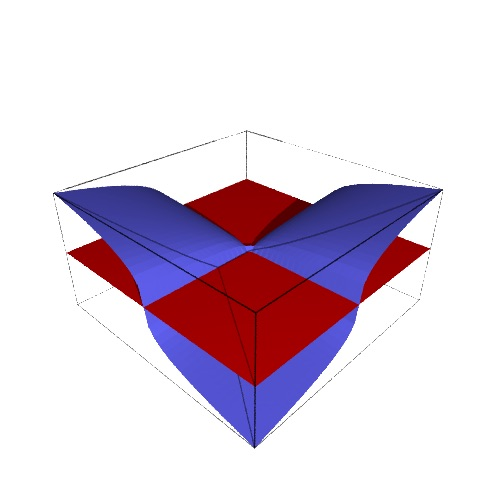
\includegraphics[scale=.5]{NonDiff}\end{center}
\end{multicols}
\end{enumerate}
\end{document}
